\documentclass[fleqn,varvw,preprintnumbers]{memo}

\usepackage[utf8]{inputenc}
\usepackage[T1]{fontenc}

\graphicspath{{../../fig/}}
\usepackage[caption=false]{subfig}
\usepackage{enumerate}

\begin{document}

\title{Memo 1: definizione degli strumenti necessari per la misura}

\author{Francesco Polleri}
\email{s5025011@studenti.unige.it}
\author{Mattia Sotgia}
\email{s4942225@studenti.unige.it}

\collaboration{Gruppo A1}
\affiliation{Dipartimento di Fisica, Università degli Studi di Genova, I-16146 Genova, Italia}

\author{Lorenzo Lucentini}
\author{Michele Giorgi}
\collaboration{Gruppo C6}
\affiliation{Dipartimento di Fisica, Università degli Studi di Genova, I-16146 Genova, Italia}

\revised{\today}
\SetBgContents{laboratorio2: Memo (dated 3 maggio 2022)}
\preprint{MEMO/1 (3 maggio 2022)}

\begin{abstract}

\end{abstract}
\maketitle

\section{Obiettivo della misurazione}

Verifica dell'effetto Hall, confronto con la previsione teorica del valore previsto di portatori di carica e misura della carica dei singoli portatori.

Definita la densità di corrente e la forza di Lorentz, abbiamo allora che la tensione di Hall si può esprimere come \begin{equation}
    V_H = \frac{iB}{wnq},\label{eq:V_H_full}
\end{equation} con $i$ corrente, $B$ campo magnetico a cui è sottoposta la sonda (fig. \ref{fig:sonda_test}) e $w$ spessore della sonda. Vediamo quindi che il valore di $n$ è facilmente ricavabile. 



\section{Definizione PLOT}

Possiamo ugualmente considerare il plot di $V_H$ come $V_H(B)$ oppure alternativamente $V_H(i)$, in entrambi i casi abbiamo dei vantaggi e degli svantaggi. Soprattutto considerando la corrente abbiamo lo svantaggio di diver trovare un modo valido per poter misurare la corrente che però non influisca in modo significativo con l'apparato sperimentale utilizzato. 
Quindi possiamo definire una funzione del tipo \begin{equation}
    V_H(B) = BC,
\end{equation} con $C$ unico parametro della funzione definito come \begin{equation}
    C=\frac{i}{wnq},
\end{equation} dove unica incognita del problema che ci poniamo di risolvere è il valore di $n$, ipotizzando come noti i valori di $q=e$, $i$ (impostata come da generatore (si veda poi tab. \ref{tab:min_max_values})) e $w$ (tabella \ref{tab:sonda}).

\section{Definizione della strumentazione necessaria}

\begin{figure*}
    \subfloat[]{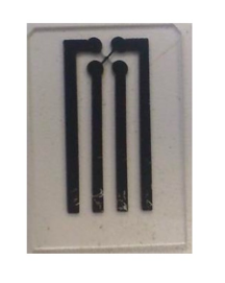
\includegraphics[]{sonda_test.pdf}\label{fig:sonda_test}}
    \subfloat[][]{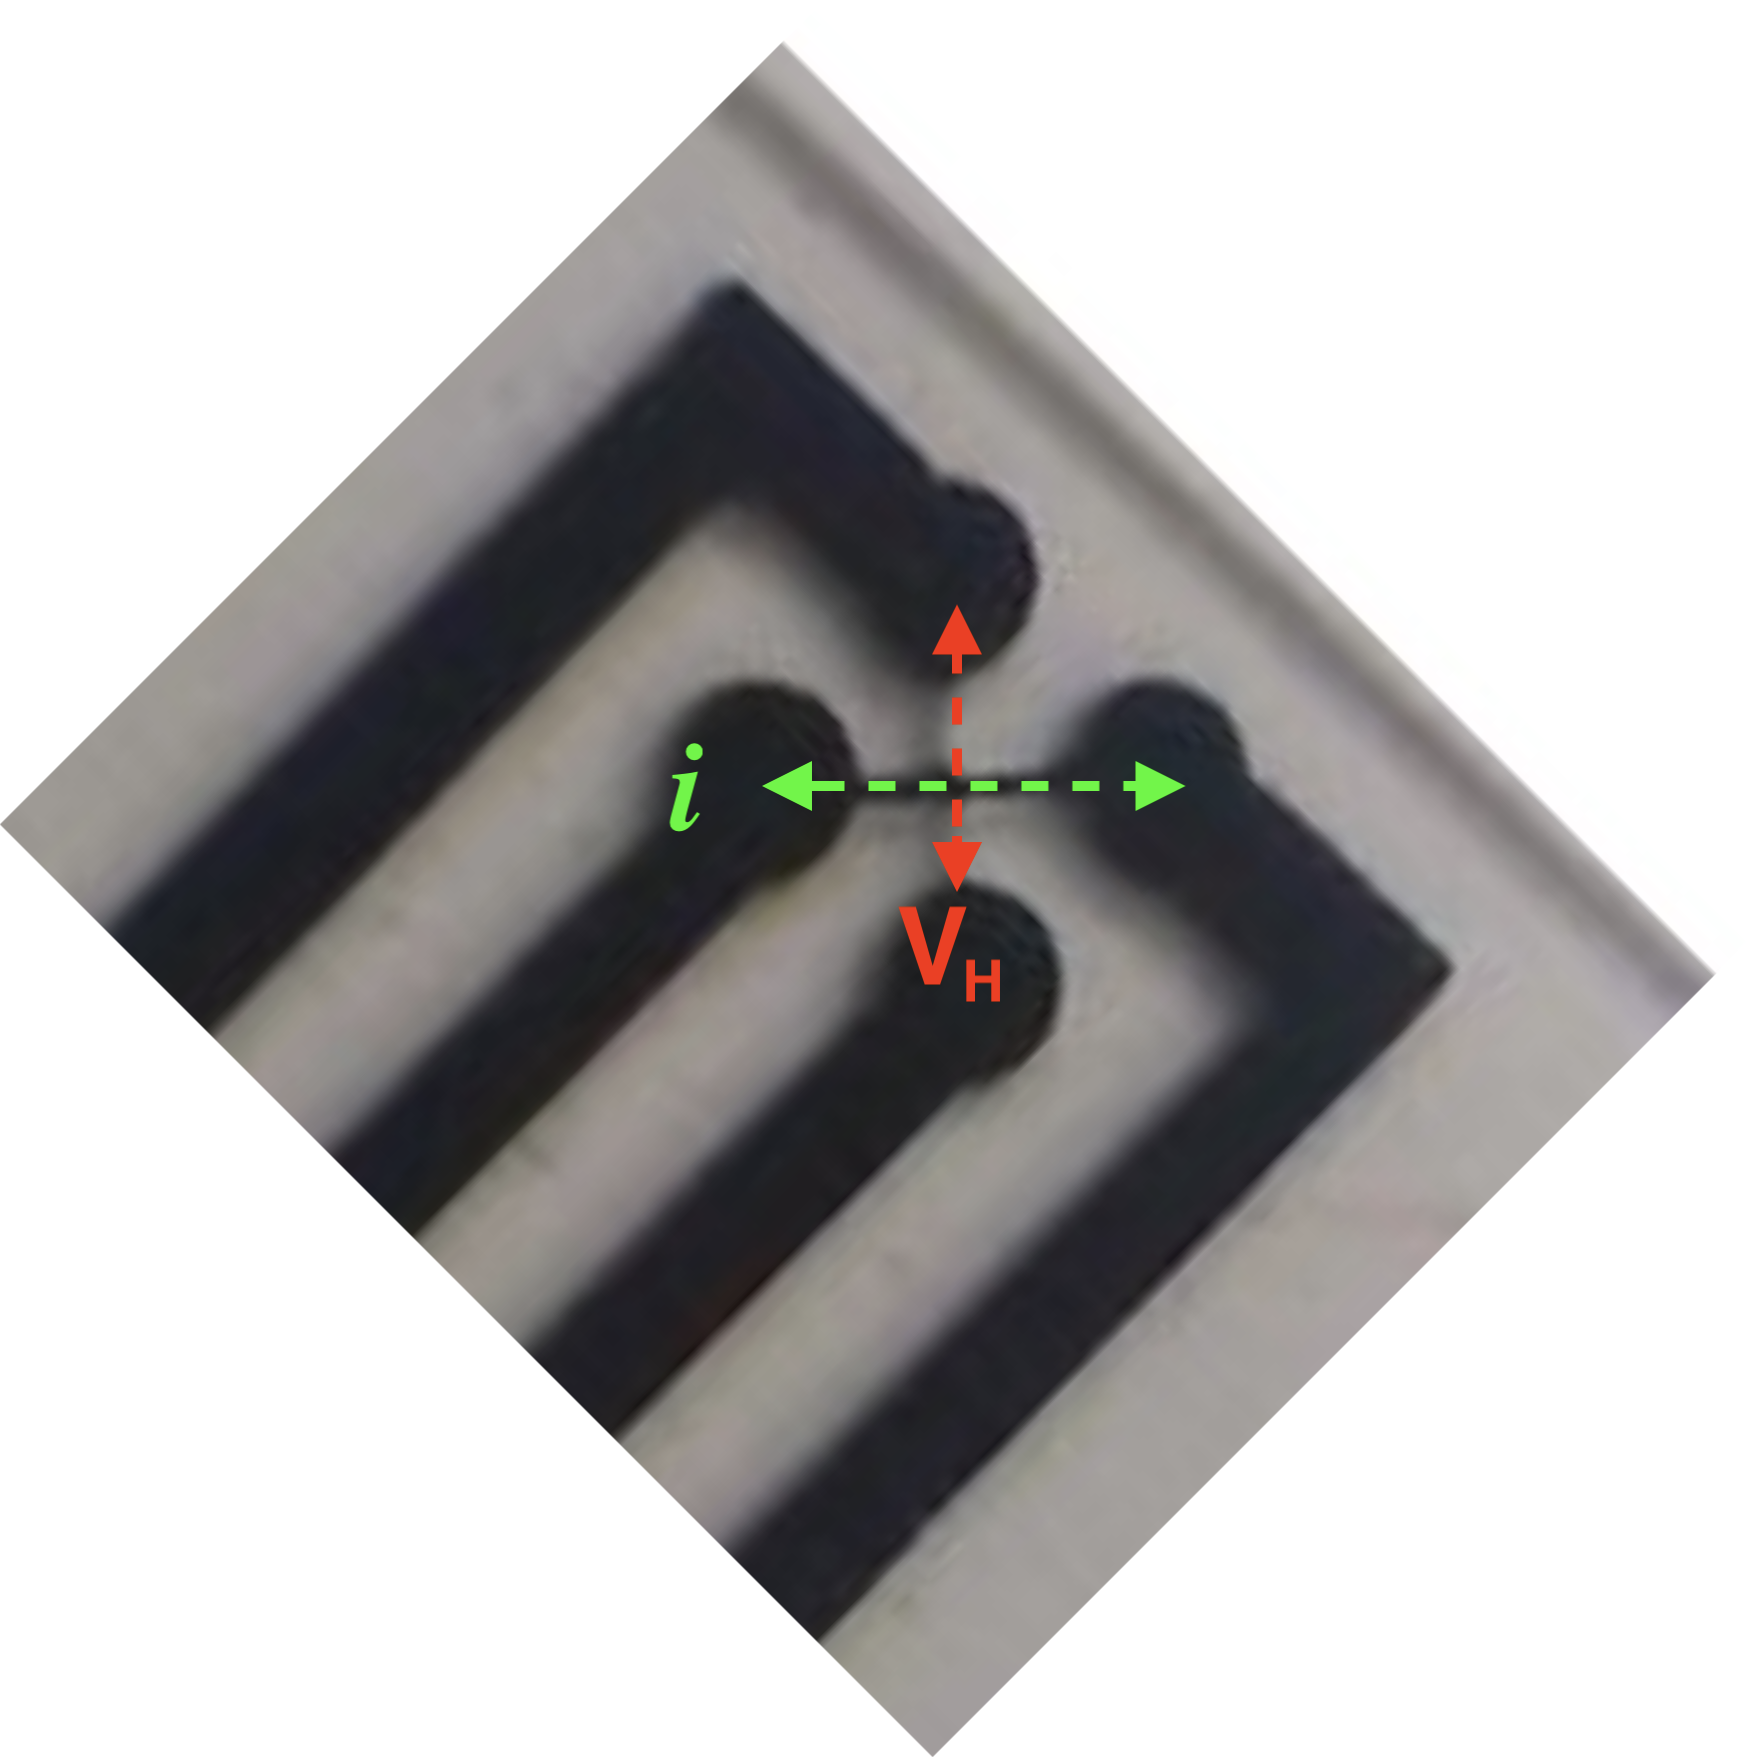
\includegraphics[width=0.25\linewidth]{zoomed_sonda.png}\label{fig:zoomed_sonda}}
    \caption{(a) Sonda utilizzata in laboratorio per la verifica dell'effetto Hall. (b) Ingrandimento ruotato di \SI{45}{\deg} della sonda sulla croce, ad indicare le direzioni di passaggio della corrente e di formazione della tensione di Hall $V_H$ (il campo magnetico è lungo la direzione ortogonale alla corrente $i$ e alla tensione $V_H$).}\label{fig:1}
\end{figure*}

\begin{table}
    \caption{(a) Dimensioni e caratteristiche della sonda utilizzata in laboratorio. (b) Alcune delle caratteristiche importanti delle strumentazioni utilizzate in laboratorio per l'esperienza. Il valore fixed value corrisponde ai casi in cui il valore della variabile non può essere cambiato, ed è limitato dalle condizioni di laboratorio (in generale indica i limiti entro cui possiamo scegliere il valore della variabile), Il valore avg. value corrisponde al valore che ricaviamo considerando sempre le limitazioni di laboratorio e che corrisponde alla miglior scelta che possiamo effettuare. \iffalse Max STD indica il valore che possiamo stimare massimo per la deviazione standard sulla misura della variabile per avere una certa risoluzione sulla nostra misura (condizioni ottimali) in parti per mille.\fi}
    \setcounter{table}{\numexpr\value{table}-1}
    \subfloat[][]{% \begin{ruledtabular}
    \begin{tabular}{lcc}
        \toprule
        MOD & Spessore $w$ (\si{\micro\metre}) & ERR (\si{\micro\metre})\\
        \colrule
        Sonda 2R & 3.3 & 0.2\\
        Sonda 6 & 12.2 & 0.6\\
        Sonda 1 & 8 & 0.5\\
        Sonda 3 & 3.8 & 0.2\\
        Sonda 2N & 6.1 & 0.3\\
        Sonda 4 & 4.5 & 0.2\\
        Sonda h5 & 3.6 & 0.2\\
        \toprule
    \end{tabular}
% \end{ruledtabular}\label{tab:sonda}}\hspace{5mm}
    \subfloat[][]{% \begin{ruledtabular}
    \begin{tabular}{lcccc}
        \toprule
        & fixed value & avg. value & max STD (ppt)\\
        \colrule
        Generatore elettrico ($i$) & - & \SI{10}{\milli\ampere} & - \\
        Campo magnetico $B$ & [0.1,0.5]\footnote{Massimo raggiungibile dagli strumenti di laboratorio, minimo importo per avere un effetto sostanzialmente utile (praticamente può andare fino a zero).} \si{\tesla} & - & - \\
        op-amp (per strum.) & - & $G\simeq 200$\footnote{Max. gain raggiungibile in condizioni di laboratorio?} & - \\
        \toprule
    \end{tabular}
% \end{ruledtabular}\label{tab:min_max_values}}
\end{table}

Abbiamo necessità di:
\begin{enumerate}[a.]
    \item un generatore di corrente
    \item un generatore di campo magnetico
    \item uno strumento per la lettura di tensione e un amplificatore differenziale
    \item un sistema di controllo per automatizzare il sistema di presa dati e controllare il setup sperimentale
    \item una sonda, che ci permetta di poter far scorrere corrente $i$ in una direzione e poter misurare nella direzione opposta la differenza di potenziale.
\end{enumerate}

\subsection{Caratterizzazione degli strumenti}
\paragraph{Generatore di corrente} Innanzitutto, per evitare di far surriscaldare la sonda, la corrente che forniamo non può avere un valore troppo alto, quindi dell'ordine di grandezza inferiore all'Ampere. Inoltre la corrente fornita alla sonda deve essere abbastanza costante, quindi non cambiare al variare della resistenza interna della sonda. Quindi sarà necessario costruire un circuito che possa permetterci di avere una corrente stabile in ingresso alla sonda, a seconda del generatore che decidiamo di utilizzare (ed in base alle disponibilità del laboratorio). 

Ipotizzando una resistenza di \SI{400}{\ohm} allora per avere una potenza dissipata piuttosto bassa (dell'ordine del \si{\milli\joule}) dobbiamo considerare correnti nell'ordine del \si{\milli\ampere}, quindi possiamo ipotizzare una corrente fornita alla sonda di \SI{10}{\milli\ampere}.

\paragraph{Generatore di campo magnetico} Possiamo utilizzare un campo magnetico creato attraverso un elettromagnete solenoidale, che rappresenta il miglior modo che abbiamo per creare un campo magnetico uniforme $B$ un una piccola e ben definita regione  di spazio. Il campo magnetico di un solenoide è \begin{equation}
    B=\frac{\mu_0iN}{\ell}. 
\end{equation} Vorremmo massimizzare il valore di $B$. Considerando le condizioni di laboratorio possiamo fissare il valore di $N/\ell$ a circa $10^4/10^5~\si{\per\metre}$, ottenendo quindi che, con una corrente di qualche decina dell'Ampere (o $10^{-1}\si{\ampere}$), il valore massimo del campo magnetico che possiamo ottenere è di $\simeq 10^{-3}/10^{-2}~\si{\tesla}$. 

L'alternativa che possiamo pensare è quella di utilizzare un circuito magnetico con traferro, che potrebbe permetterci di ottenere campi di intensità maggiore, quindi nell'ordine di \SI{0.5}{\tesla} al massimo. Possiamo quindi ipotizzare di ottenere un campo magnetico di circa \SI{0.3}{\tesla} utilizzando un circuito magnetico e misurando il campo nel traferro.

\paragraph{Lettura di tensione} Ai capi della sonda vogliamo misurare la tensione di Hall $V_H$, quindi abbiamo bisogno di uno strumento che abbia la possibilità di leggere la tensione ai capi della sonda. La tensione di Hall risulterà essere però molto bassa, infatti con le quantità fornite fino ad ora possiamo ipotizzare che sia necessario amplificarlo. L'amplificatore migliore che possiamo realizzare può avere un valore di circa 100/400, per esempio utilizzando un amplificatore per strumentazione diviso in due fasi, la prima con guadagno 10/20 e la seconda con un guadagno simile. Quindi abbiamo bisogno di uno strumento per la lettura della tensione piuttosto preciso, che possa leggere differenze di potenziale dell'ordine del \si{\milli\volt}. 

\paragraph{Sistema di controllo} Vogliamo poi avere un sistema centrale che ci permetta di controllare la logica del setup sperimentale e che permetta di mettere in comunicazione i vari strumenti e attivarli con impostazioni ben definite e poter effettuare misure in modo automatico. Viene comodo quindi utilizzare un sistema integrato come Arduino, per cui possiamo realizzare una logica semplice per controllare il setup sperimentale e per raccogliere misure. 

\paragraph{Sonda} Con i dati fino ad ora raccolti ci possiamo accorgere che la tensione di Hall dipende fortemente dal numero di portatori, e vogliamo che infatti sia un valore più basso possibile, per ottenere tensioni misurabili più alte possibili (\emph{cfr.} eq. (\ref{eq:V_H_full})). Vogliamo quindi trovare un materiale che abbia un buon compromesso tra la resistenza interna e il numero di portatori, in modo da ottenere un valore della tensione di Hall più alto possibile, senza dover però fornire correnti eccessivamente basse, difficili da generare, e che causerebbero un valore della tensione di Hall ancora più bassa. Il materiale che abbiamo a disposizione è il rame, depositato a formare uno strat laminare molto sottile per cui possiamo identificare delle direzioni privilegiate per la corrente e per la valutazione dell'effetto Hall. 

\end{document}